\chapter{Overview della webapp}

\section{Login}
All'accesso della webapp viene mostrata la pagina di login, in cui è possibile inserire le proprie credenziali per accedere al sistema. \ref{fig:login}.

\begin{figure}[ht]
    \centering
    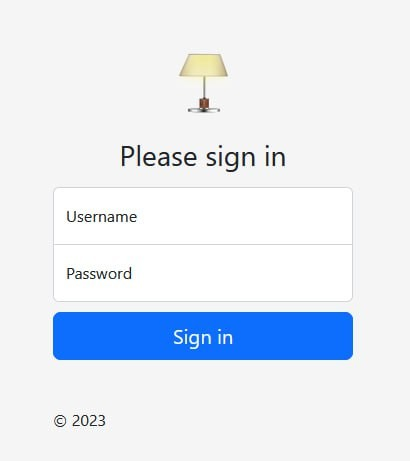
\includegraphics[width=0.4\textwidth]{img/login.jpg}
    \caption{Immagine della pagina di login.}
    \label{fig:login}
\end{figure}

\section{Pagine webapp}

Dopo aver eseguito il login, l'utente viene reindirizzato alla pagina \textit{Dashboard lampioni} che fungerà da pagina principale della webapp. Utilizzando i bottoni presenti nell'header della pagina sarà possibile spostarsi tra le varie pagine disponibili.

\section{Dashboard Lampioni}

Pagina in cui si viene automaticamente reindirizzati una volta eseguito il login, è inoltre possibile accedere a questa pagina premendo il relativo pulsante nell'header della pagina. In questa pagina vengono mostrati tutti i lampioni presenti a sistema e le loro informazioni. Inoltre è possibile impostare una luminosità specifica su ognuno di essi. Per applicare le modifiche basterà premere il pulsante conferma relativo al lampione desiderato. \ref{fig:lista_lampioni}.

\begin{figure}[ht]
    \centering
    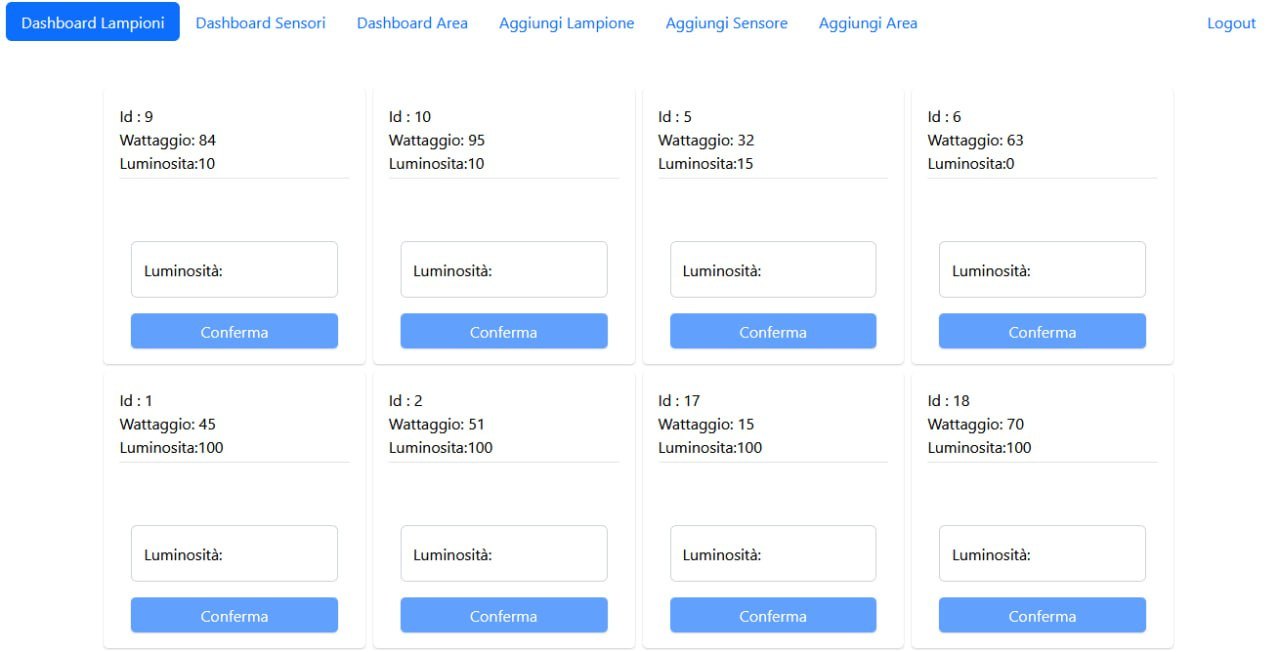
\includegraphics[width=\textwidth]{img/lista_lampioni.jpeg}
    \caption{Immagine della pagina Dashboard Lampioni.}
    \label{fig:lista_lampioni}
\end{figure}

\section{Dashboard Sensori}

Per accedere a questa pagina bisogna premere il relativo pulsante nell'header della pagina. In questa pagina vengono mostrati tutti i sensori presenti a sistema e le loro relative informazioni \ref{fig:lista_sensori}.

\begin{figure}[ht]
    \centering
    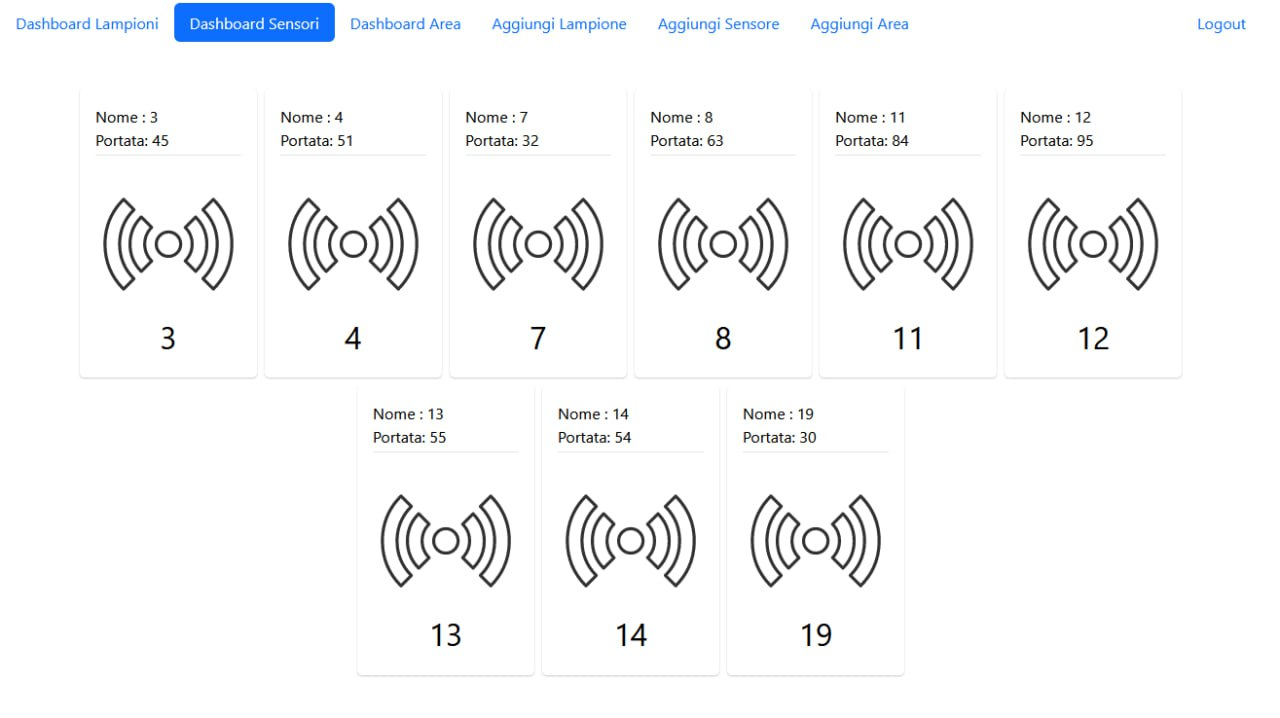
\includegraphics[width=\textwidth]{img/lista_sensori.jpeg}
    \caption{Immagine della pagina Dashboard Sensori.}
    \label{fig:lista_sensori}
\end{figure}

\section{Dashboard Area}

Per accedere a questa pagina bisogna premere il relativo pulsante nell'header della pagina. In questa pagina vengono mostrate tutte le aree presenti a sistema e le relative informazioni \ref{fig:lista_area}.

\begin{figure}[ht]
    \centering
    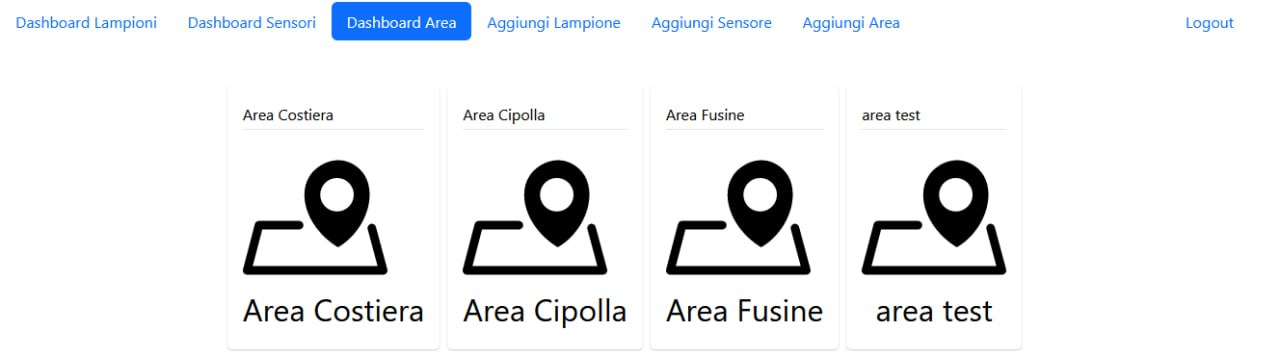
\includegraphics[width=\textwidth]{img/lista_area.jpeg}
    \caption{Immagine della pagina Dashboard Area.}
    \label{fig:lista_area}
\end{figure}

\section{Aggiungi Lampione}

Per accedere a questa pagina bisogna premere il relativo pulsante nell'header della pagina. In questa pagina è presente un form che permette di aggiungere un lampione a sistema digitando nei relativi campi le informazioni relative al lampione (idArea, latitudine, longitudine e wattaggio). Premendo il pulsante conferma si effettua l'aggiunta a sistema del lampione desiderato \ref{fig:aggiunta_lamp}.

\begin{figure}[ht]
    \centering
    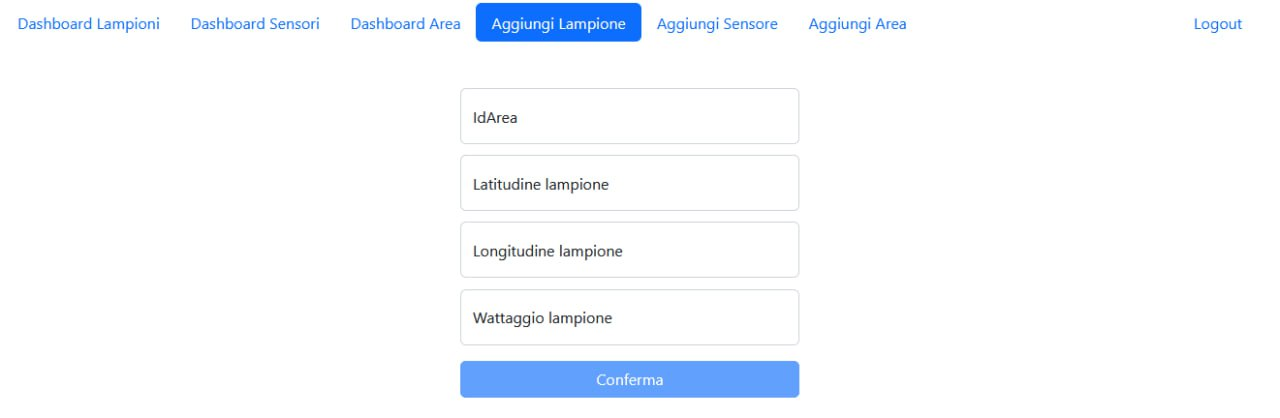
\includegraphics[width=\textwidth]{img/aggiunta_lamp.jpeg}
    \caption{Immagine della pagina Aggiungi Lampioni.}
    \label{fig:aggiunta_lamp}
\end{figure}

\section{Aggiungi Sensore}

Per accedere a questa pagina bisogna premere il relativo pulsante nell'header della pagina. In questa pagina è presente un form che permette di aggiungere un sensore a sistema digitando nei relativi campi le informazioni relative al sensore (idArea, latitudine, longitudine e raggio). Premendo il pulsante conferma si effettua l'aggiunta a sistema del sensore desiderato \ref{fig:aggiunta_sens}.

\begin{figure}[ht]
    \centering
    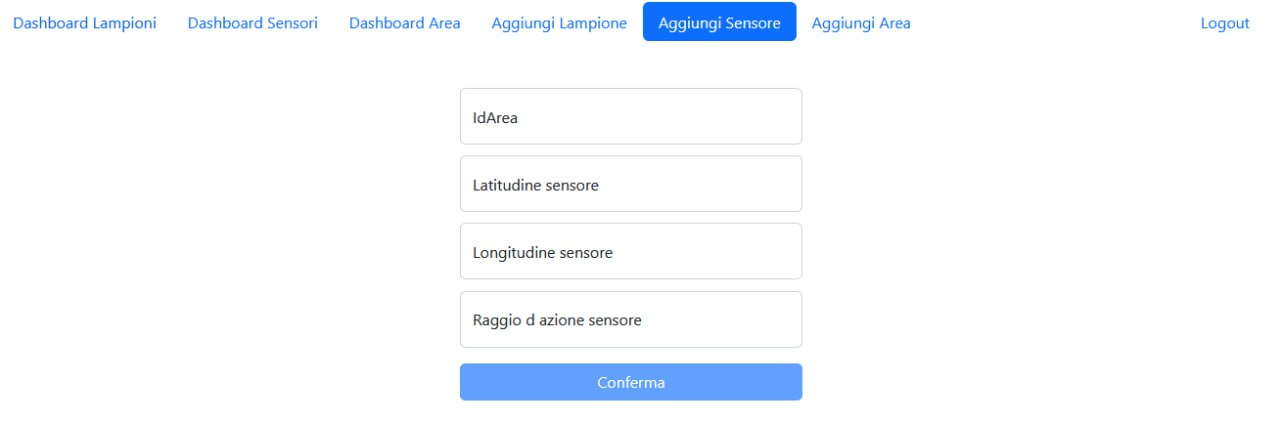
\includegraphics[width=\textwidth]{img/aggiunta_sens.jpeg}
    \caption{Immagine della pagina Aggiungi Sensori.}
    \label{fig:aggiunta_sens}
\end{figure}

\section{Aggiungi Area}

Per accedere a questa pagina bisogna premere il relativo pulsante nell'header della pagina. In questa pagina è presente un form che permette di aggiungere un' area a sistema digitando nei relativi campi le informazioni relative all'area (Alias). Premendo il pulsante conferma si effettua l'aggiunta a sistema dell'area desiderata \ref{fig:aggiunta_area}.

\begin{figure}[ht]
    \centering
    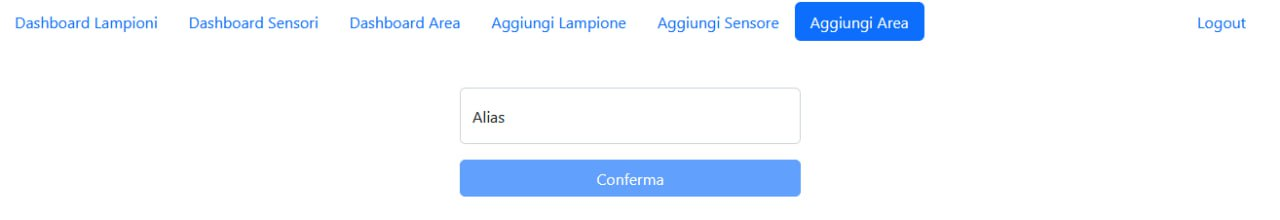
\includegraphics[width=\textwidth]{img/aggiunta_area.jpeg}
    \caption{Immagine della pagina Aggiungi Area.}
    \label{fig:aggiunta_area}
\end{figure}

\section{Logout}

Per disconnettersi dal proprio account basterà premere il pulsante \textit{Logout} presente nell'header della pagina.